\documentclass[12pt]{article}
%\usepackage[utf8]{inputenc}
%\documentclass[UTF8]{ctexart}
%\usepackage[UTF8, heading = false, scheme = plain]{ctex}
\usepackage{geometry}
%geometry{a4paper,scale=0.9}
\geometry{a4paper,left=1cm,right=1cm,top=1cm,bottom=2cm}
\usepackage{amsfonts}
\usepackage{color}
\usepackage{url}
%\usepackage{biblatex}
\usepackage{amsmath}
\usepackage{amssymb}
\usepackage{latexsym}
\usepackage{cite}
%\addbibresource{ref.bib}
%\bibliography{ref.bib}
\usepackage{caption}
\usepackage{graphicx, subfig}
\usepackage{float}
%\usepackage[fontset=ubuntu]{ctex}
%\usepackage{fontspec}
\usepackage{xeCJK}
%\usepackage[colorlinks,
%anchorcolor=black,
%citecolor=black]{hyperref}
%\setmainfont{SimSun}
\usepackage[section]{placeins}
\usepackage{enumitem}
\usepackage{framed}
\usepackage[framemethod=TikZ]{mdframed}
\usepackage{indentfirst}
\usepackage{setspace}%使用间距宏包
\linespread{1.5}

\title{一致性哈希\cite{For_Interview_What_Is_Consistent_Hashing}}
\author{leolinuxer}
%\date{June 2020}

\begin{document}
%\setlength{\parindent}{0pt}
\maketitle
\tableofcontents

\section{一致性哈希的直观理解}
\subsection{Redis集群的使用}
我们在使用Redis的时候,为了保证Redis的高可用,提高Redis的读写性能,最简单的方式我们会做主从复制,组成Master-Master或者Master-Slave的形式,或者搭建Redis集群,进行数据的读写分离,类似于数据库的主从复制和读写分离。如下所示:
\begin{figure}[H]
    \centering
    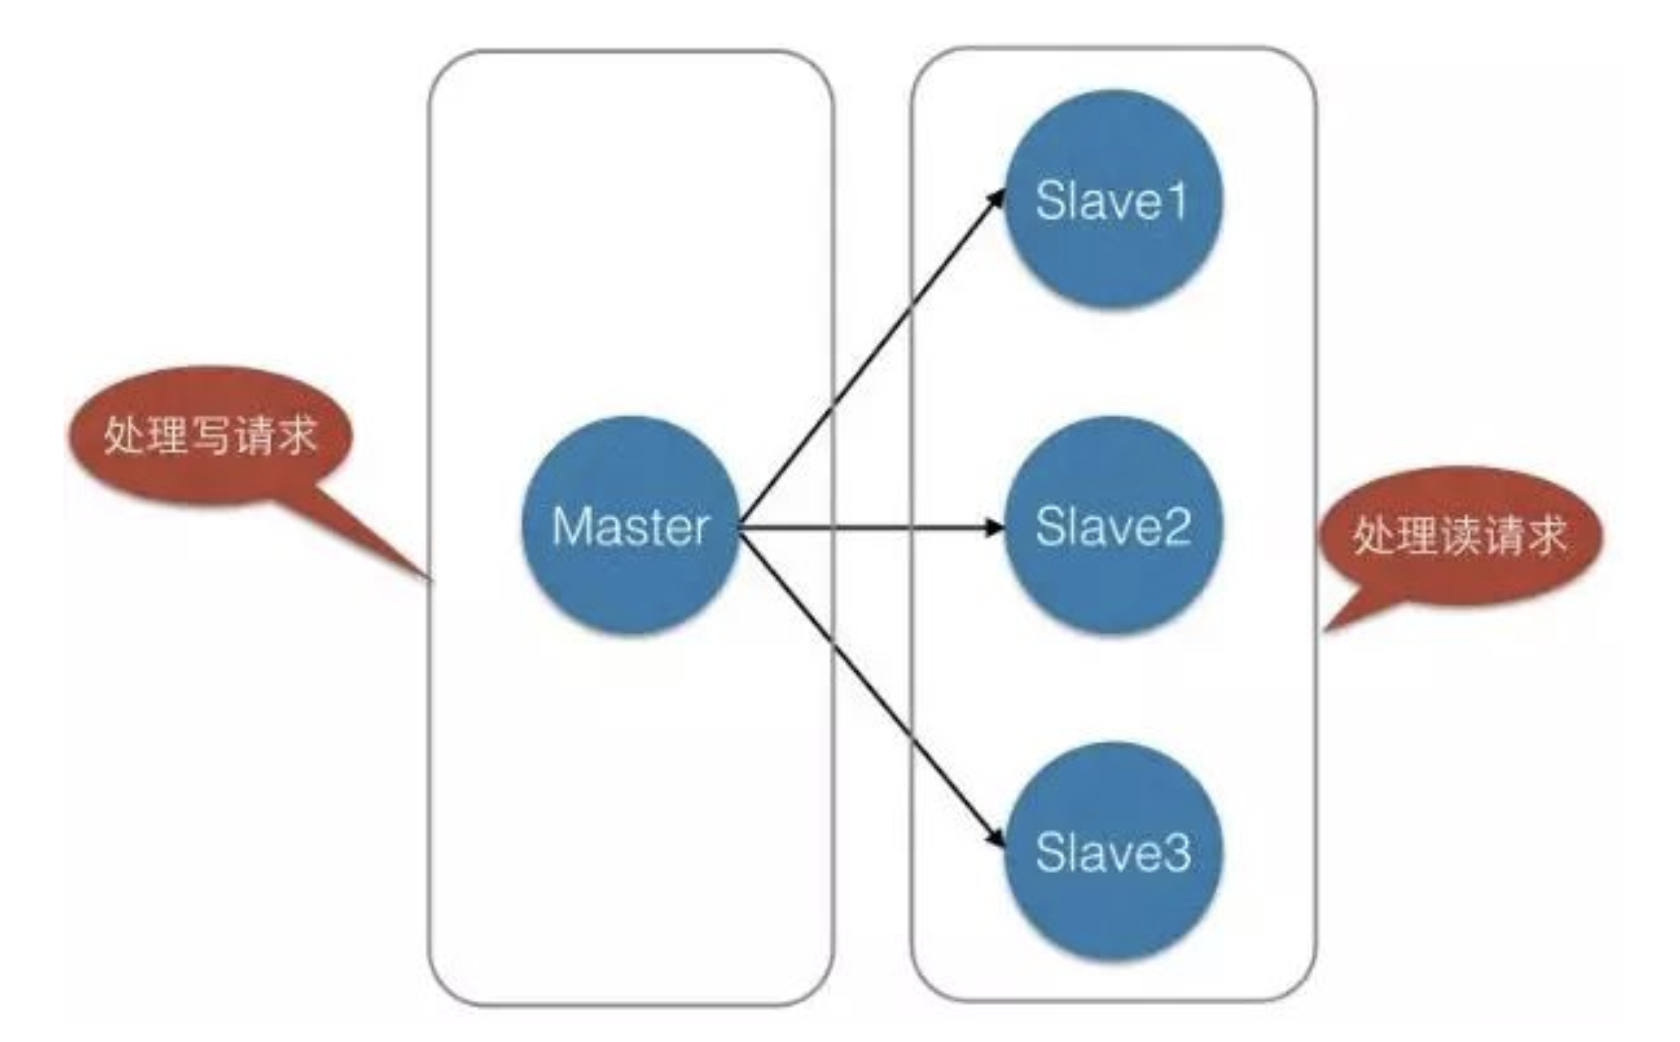
\includegraphics[width=.4\textwidth]{fig/Consistent_Hashing_1.png}
\end{figure}

同样类似于数据库,当单表数据大于500W的时候需要对其进行分库分表,当数据量很大的时候(标准可能不一样,要看Redis服务器容量)我们同样可以对Redis进行类似的操作,就是分库分表。

假设,我们有一个社交网站,需要使用Redis存储图片资源,存储的格式为键值对,key值为图片名称,value为该图片所在文件服务器的路径,我们需要根据文件名查找该文件所在文件服务器上的路径,数据量大概有2000W左右,按照我们约定的规则进行分库,规则就是随机分配,我们可以部署8台缓存服务器,每台服务器大概含有500W条数据,并且进行主从复制,示意图如下:
\begin{figure}[H]
    \centering
    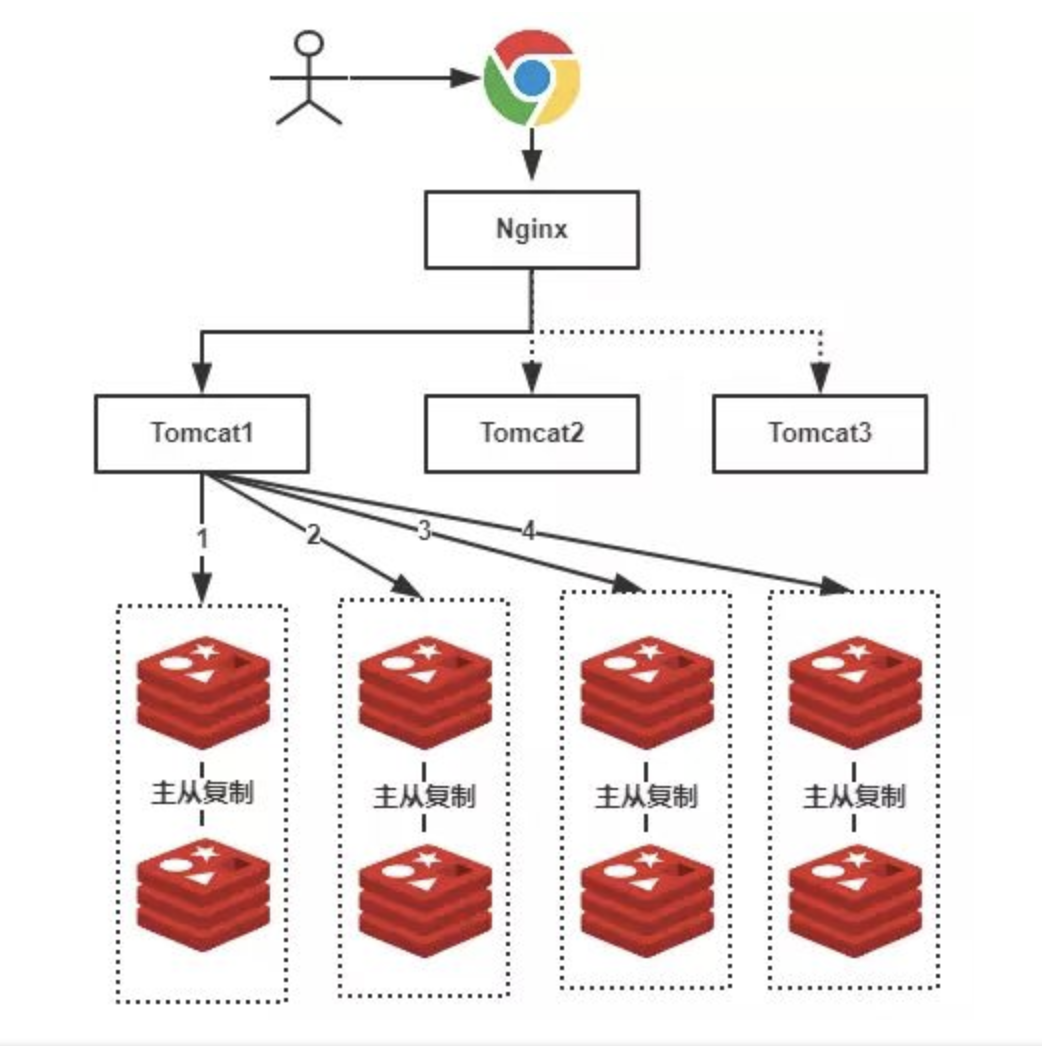
\includegraphics[width=.4\textwidth]{fig/Consistent_Hashing_2.png}
\end{figure}

由于规则是随机的,所有我们的一条数据都有可能存储在任何一组Redis中,例如上图我们用户查找一张名称为”a.png”的图片,由于规则是随机的,我们不确定具体是在哪一个Redis服务器上的,因此我们需要进行1、2、3、4,4次查询才能够查询到(也就是遍历了所有的Redis服务器),这显然不是我们想要的结果,有了解过的小伙伴可能会想到,随机的规则不行,可以使用类似于数据库中的分库分表规则:按照Hash值、取模、按照类别、按照某一个字段值等等常见的规则就可以出来了!好,按照我们的主题,我们就使用Hash的方式。

\subsection{为Redis集群使用Hash}
可想而知,如果我们使用Hash的方式,每一张图片在进行分库的时候都可以定位到特定的服务器,示意图如下:
\begin{figure}[H]
    \centering
    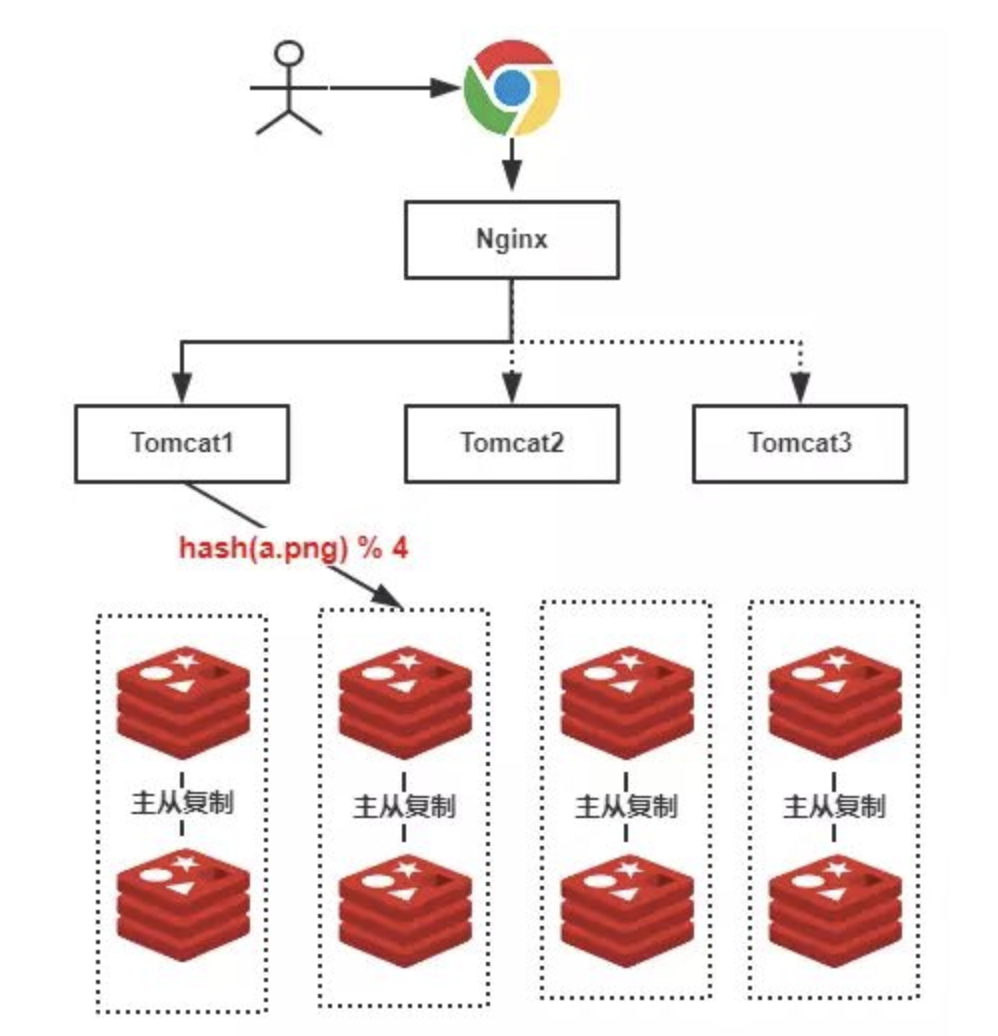
\includegraphics[width=.4\textwidth]{fig/Consistent_Hashing_3.png}
\end{figure}

上图中,假设我们查找的是”a.png”,由于有4台服务器(排除从库),因此公式为hash(a.png) \% 4 = 2 ,可知定位到了第2号服务器,这样的话就不会遍历所有的服务器,大大提升了性能!

\subsection{使用Hash的问题}
上述的方式虽然提升了性能,我们不再需要对整个Redis服务器进行遍历!但是,使用上述Hash算法进行缓存时,会出现一些缺陷,主要体现在服务器数量变动的时候,所有缓存的位置都要发生改变!

试想一下,如果4台缓存服务器已经不能满足我们的缓存需求,那么我们应该怎么做呢?很简单,多增加几台缓存服务器不就行了!假设:我们增加了一台缓存服务器,那么缓存服务器的数量就由4台变成了5台。那么原本hash(a.png) \% 4 = 2 的公式就变成了hash(a.png) \% 5 = ? , 可想而知这个结果肯定不是2的,这种情况带来的结果就是当服务器数量变动时,所有缓存的位置都要发生改变!换句话说,当服务器数量发生改变时,所有缓存在一定时间内是失效的,当应用无法从缓存中获取数据时,则会向后端数据库请求数据!

同样的,假设4台缓存中突然有一台缓存服务器出现了故障,无法进行缓存,那么我们则需要将故障机器移除,但是如果移除了一台缓存服务器,那么缓存服务器数量从4台变为3台,也是会出现上述的问题!

所以,我们应该想办法不让这种情况发生,但是由于上述Hash算法本身的缘故,使用取模法进行缓存时,这种情况是无法避免的,为了解决这些问题,Hash一致性算法(一致性Hash算法)诞生了!

\subsection{一致性Hash算法的神秘面纱}
一致性Hash算法也是使用取模的方法,只是,刚才描述的取模法是对服务器的数量进行取模,而一致性Hash算法是对$2^32$取模,什么意思呢?简单来说,一致性Hash算法将整个哈希值空间组织成一个虚拟的圆环,如假设某哈希函数H的值空间为$0-2^32-1$(即哈希值是一个32位无符号整形),整个哈希环如下:
\begin{figure}[H]
    \centering
    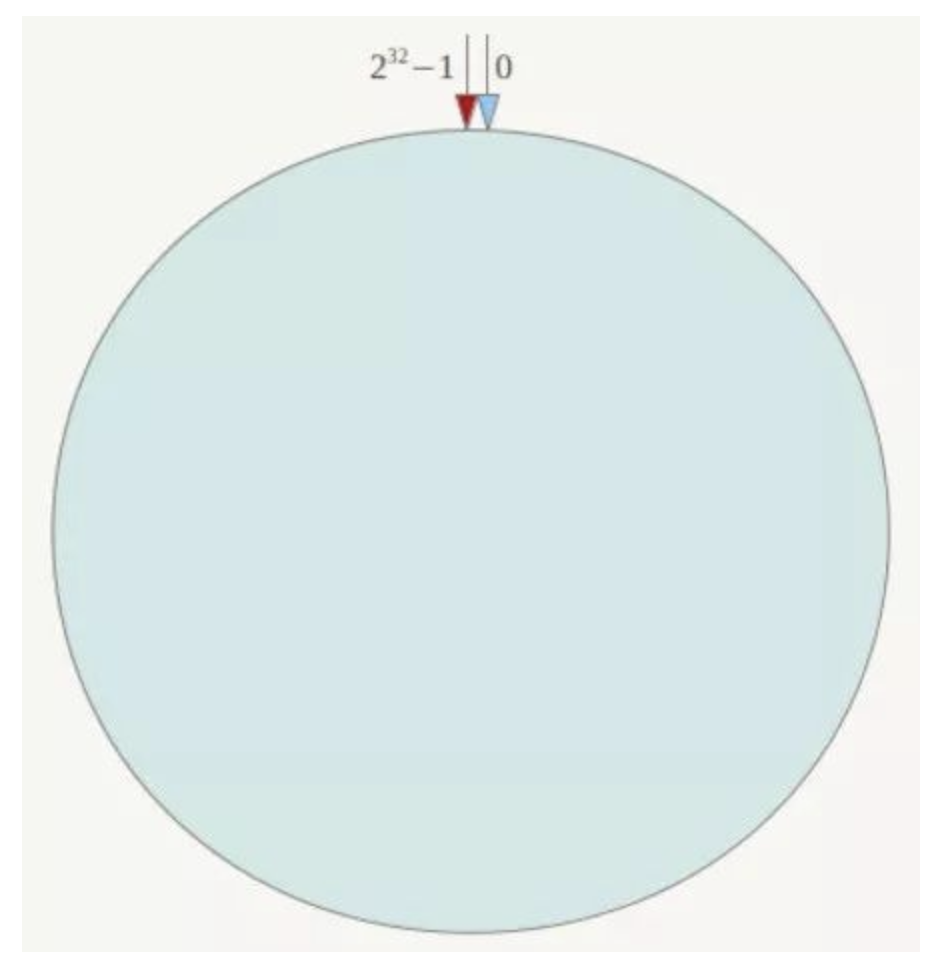
\includegraphics[width=.4\textwidth]{fig/Consistent_Hashing_4.png}
\end{figure}
整个空间按顺时针方向组织,圆环的正上方的点代表0,0点右侧的第一个点代表1,以此类推,2、3、4、5、6……直到$2^32-1$,也就是说0点左侧的第一个点代表$2^32-1$, 0和$2^32-1$在零点中方向重合,我们把这个由$2^32$个点组成的圆环称为Hash环。

下一步将各个服务器使用Hash进行一个哈希,具体可以选择服务器的IP或主机名作为关键字进行哈希,这样每台机器就能确定其在哈希环上的位置,这里假设将上文中四台服务器使用IP地址哈希后在环空间的位置如下:
\begin{figure}[H]
    \centering
    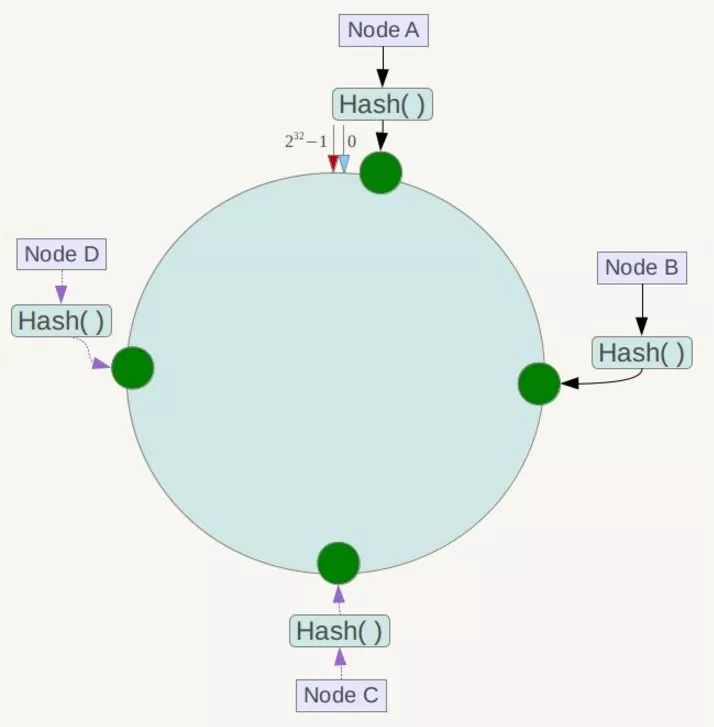
\includegraphics[width=.5\textwidth]{fig/Consistent_Hashing_6.jpg}
\end{figure}

接下来使用如下算法定位数据访问到相应服务器:将数据key使用相同的函数Hash计算出哈希值,并确定此数据在环上的位置,从此位置沿环顺时针“行走”,第一台遇到的服务器就是其应该定位到的服务器!

例如我们有Object A、Object B、Object C、Object D四个数据对象,经过哈希计算后,在环空间上的位置如下:
\begin{figure}[H]
    \centering
    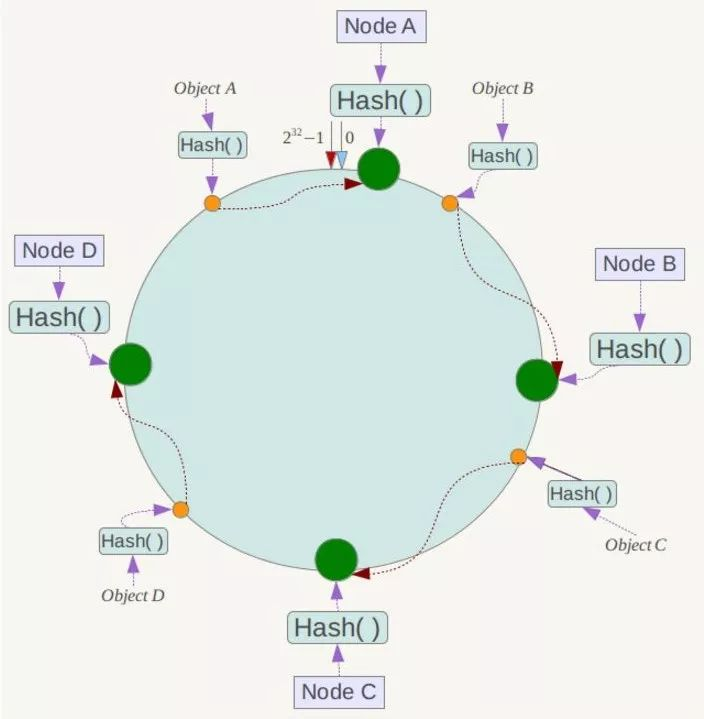
\includegraphics[width=.5\textwidth]{fig/Consistent_Hashing_7.jpg}
\end{figure}

根据一致性Hash算法,数据A会被定为到Node A上,B被定为到Node B上,C被定为到Node C上,D被定为到Node D上。

\subsection{一致性Hash算法的容错性和可扩展性}
现假设Node C不幸宕机,可以看到此时对象A、B、D不会受到影响,只有C对象被重定位到Node D。一般的,在一致性Hash算法中,如果一台服务器不可用,则受影响的数据仅仅是此服务器到其环空间中前一台服务器(即沿着逆时针方向行走遇到的第一台服务器)之间数据,其它不会受到影响,如下所示:
\begin{figure}[H]
    \centering
    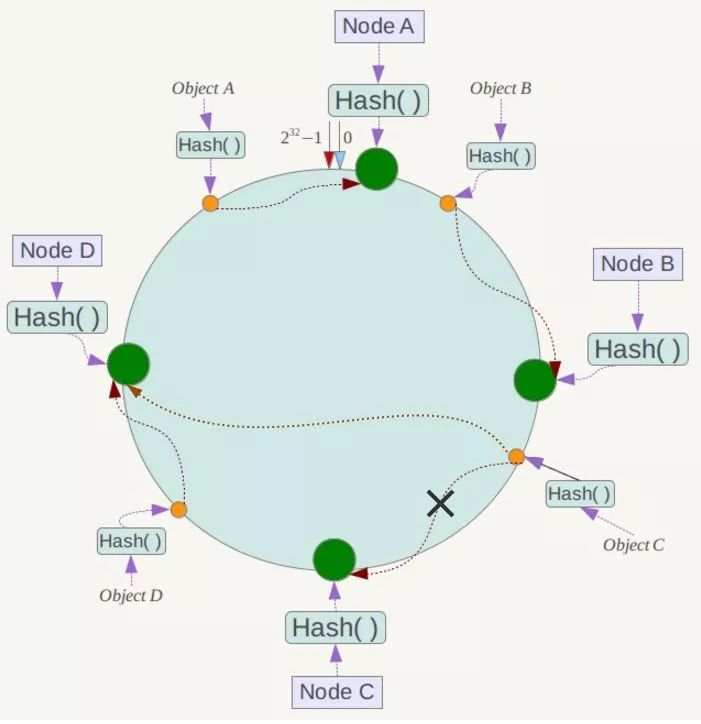
\includegraphics[width=.5\textwidth]{fig/Consistent_Hashing_8.jpg}
\end{figure}

下面考虑另外一种情况,如果在系统中增加一台服务器Node X,如下图所示:
\begin{figure}[H]
    \centering
    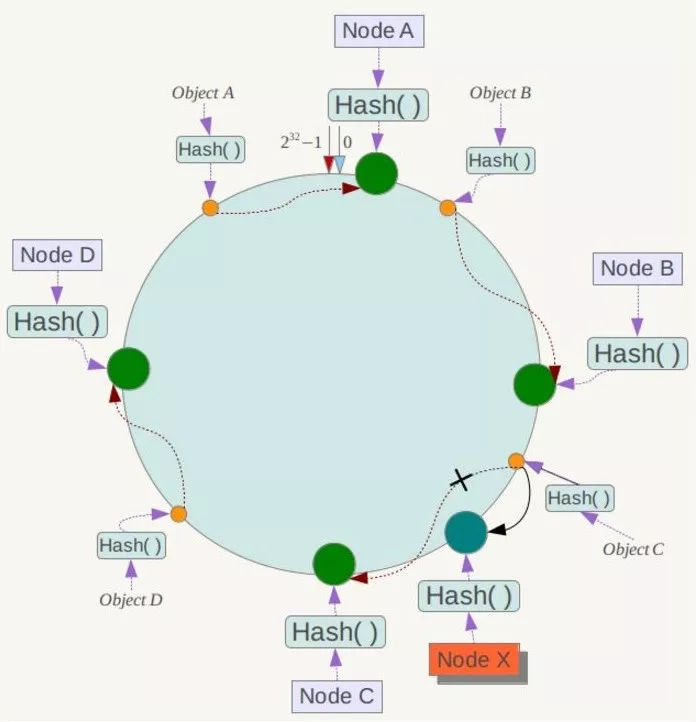
\includegraphics[width=.5\textwidth]{fig/Consistent_Hashing_9.jpg}
\end{figure}

此时对象Object A、B、D不受影响,只有对象C需要重定位到新的Node X !一般的,在一致性Hash算法中,如果增加一台服务器,则受影响的数据仅仅是新服务器到其环空间中前一台服务器(即沿着逆时针方向行走遇到的第一台服务器)之间数据,其它数据也不会受到影响。

综上所述,一致性Hash算法对于节点的增减都只需重定位环空间中的一小部分数据,具有较好的容错性和可扩展性。

\subsection{Hash环的数据倾斜问题}
一致性Hash算法在服务节点太少时,容易因为节点分部不均匀而造成数据倾斜(被缓存的对象大部分集中缓存在某一台服务器上)问题,例如系统中只有两台服务器,其环分布如下:
\begin{figure}[H]
    \centering
    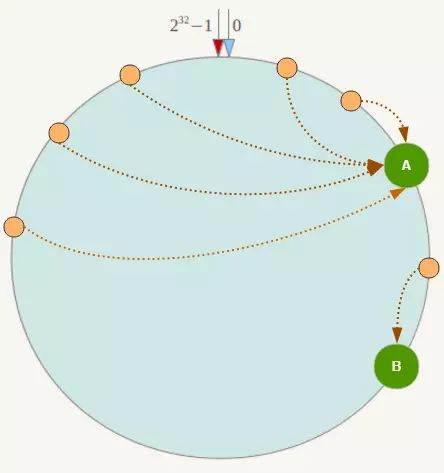
\includegraphics[width=.5\textwidth]{fig/Consistent_Hashing_10.jpg}
\end{figure}

此时必然造成大量数据集中到Node A上,而只有极少量会定位到Node B上。为了解决这种数据倾斜问题,一致性Hash算法引入了虚拟节点机制,即对每一个服务节点计算多个哈希,每个计算结果位置都放置一个此服务节点,称为虚拟节点。具体做法可以在服务器IP或主机名的后面增加编号来实现。

例如上面的情况,可以为每台服务器计算三个虚拟节点,于是可以分别计算 “Node A\#1”、“Node A\#2”、“Node A\#3”、“Node B\#1”、“Node B\#2”、“Node B\#3”的哈希值,于是形成六个虚拟节点:
\begin{figure}[H]
    \centering
    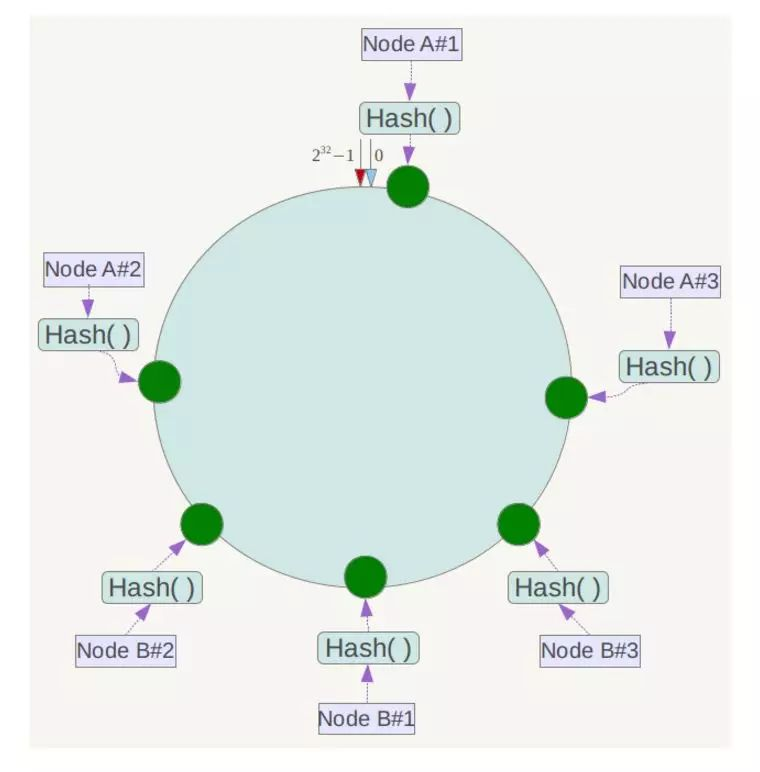
\includegraphics[width=.5\textwidth]{fig/Consistent_Hashing_11.jpg}
\end{figure}

同时数据定位算法不变,只是多了一步虚拟节点到实际节点的映射,例如定位到“Node A\#1”、“Node A\#2”、“Node A\#3”三个虚拟节点的数据均定位到Node A上。这样就解决了服务节点少时数据倾斜的问题。在实际应用中,通常将虚拟节点数设置为32甚至更大,因此即使很少的服务节点也能做到相对均匀的数据分布。



%\printbibliography
\bibliography{../ref}
\bibliographystyle{IEEEtran}
\end{document}